%% bare_conf_compsoc.tex
%% V1.4b
%% 2015/08/26
%% by Michael Shell
%% See:
%% http://www.michaelshell.org/
%% for current contact information.
%%
%% This is a skeleton file demonstrating the use of IEEEtran.cls
%% (requires IEEEtran.cls version 1.8b or later) with an IEEE Computer
%% Society conference paper.
%%
%% Support sites:
%% http://www.michaelshell.org/tex/ieeetran/
%% http://www.ctan.org/pkg/ieeetran
%% and
%% http://www.ieee.org/

%%*************************************************************************
%% Legal Notice:
%% This code is offered as-is without any warranty either expressed or
%% implied; without even the implied warranty of MERCHANTABILITY or
%% FITNESS FOR A PARTICULAR PURPOSE! 
%% User assumes all risk.
%% In no event shall the IEEE or any contributor to this code be liable for
%% any damages or losses, including, but not limited to, incidental,
%% consequential, or any other damages, resulting from the use or misuse
%% of any information contained here.
%%
%% All comments are the opinions of their respective authors and are not
%% necessarily endorsed by the IEEE.
%%
%% This work is distributed under the LaTeX Project Public License (LPPL)
%% ( http://www.latex-project.org/ ) version 1.3, and may be freely used,
%% distributed and modified. A copy of the LPPL, version 1.3, is included
%% in the base LaTeX documentation of all distributions of LaTeX released
%% 2003/12/01 or later.
%% Retain all contribution notices and credits.
%% ** Modified files should be clearly indicated as such, including  **
%% ** renaming them and changing author support contact information. **
%%*************************************************************************


% *** Authors should verify (and, if needed, correct) their LaTeX system  ***
% *** with the testflow diagnostic prior to trusting their LaTeX platform ***
% *** with production work. The IEEE's font choices and paper sizes can   ***
% *** trigger bugs that do not appear when using other class files.       ***                          ***
% The testflow support page is at:
% http://www.michaelshell.org/tex/testflow/



\documentclass[conference,compsoc]{IEEEtran}
% Some/most Computer Society conferences require the compsoc mode option,
% but others may want the standard conference format.
%
% If IEEEtran.cls has not been installed into the LaTeX system files,
% manually specify the path to it like:
% \documentclass[conference,compsoc]{../sty/IEEEtran}





% Some very useful LaTeX packages include:
% (uncomment the ones you want to load)


% *** MISC UTILITY PACKAGES ***
%
%\usepackage{ifpdf}
% Heiko Oberdiek's ifpdf.sty is very useful if you need conditional
% compilation based on whether the output is pdf or dvi.
% usage:
% \ifpdf
%   % pdf code
% \else
%   % dvi code
% \fi
% The latest version of ifpdf.sty can be obtained from:
% http://www.ctan.org/pkg/ifpdf
% Also, note that IEEEtran.cls V1.7 and later provides a builtin
% \ifCLASSINFOpdf conditional that works the same way.
% When switching from latex to pdflatex and vice-versa, the compiler may
% have to be run twice to clear warning/error messages.






% *** CITATION PACKAGES ***
%
\ifCLASSOPTIONcompsoc
  % IEEE Computer Society needs nocompress option
  % requires cite.sty v4.0 or later (November 2003)
  \usepackage[nocompress]{cite}
\else
  % normal IEEE
  \usepackage{cite}
\fi
% cite.sty was written by Donald Arseneau
% V1.6 and later of IEEEtran pre-defines the format of the cite.sty package
% \cite{} output to follow that of the IEEE. Loading the cite package will
% result in citation numbers being automatically sorted and properly
% "compressed/ranged". e.g., [1], [9], [2], [7], [5], [6] without using
% cite.sty will become [1], [2], [5]--[7], [9] using cite.sty. cite.sty's
% \cite will automatically add leading space, if needed. Use cite.sty's
% noadjust option (cite.sty V3.8 and later) if you want to turn this off
% such as if a citation ever needs to be enclosed in parenthesis.
% cite.sty is already installed on most LaTeX systems. Be sure and use
% version 5.0 (2009-03-20) and later if using hyperref.sty.
% The latest version can be obtained at:
% http://www.ctan.org/pkg/cite
% The documentation is contained in the cite.sty file itself.
%
% Note that some packages require special options to format as the Computer
% Society requires. In particular, Computer Society  papers do not use
% compressed citation ranges as is done in typical IEEE papers
% (e.g., [1]-[4]). Instead, they list every citation separately in order
% (e.g., [1], [2], [3], [4]). To get the latter we need to load the cite
% package with the nocompress option which is supported by cite.sty v4.0
% and later.





% *** GRAPHICS RELATED PACKAGES ***
%
\ifCLASSINFOpdf
  % \usepackage[pdftex]{graphicx}
  % declare the path(s) where your graphic files are
  % \graphicspath{{../pdf/}{../jpeg/}}
  % and their extensions so you won't have to specify these with
  % every instance of \includegraphics
  % \DeclareGraphicsExtensions{.pdf,.jpeg,.png}
\else
  % or other class option (dvipsone, dvipdf, if not using dvips). graphicx
  % will default to the driver specified in the system graphics.cfg if no
  % driver is specified.
  % \usepackage[dvips]{graphicx}
  % declare the path(s) where your graphic files are
  % \graphicspath{{../eps/}}
  % and their extensions so you won't have to specify these with
  % every instance of \includegraphics
  % \DeclareGraphicsExtensions{.eps}
\fi
% graphicx was written by David Carlisle and Sebastian Rahtz. It is
% required if you want graphics, photos, etc. graphicx.sty is already
% installed on most LaTeX systems. The latest version and documentation
% can be obtained at: 
% http://www.ctan.org/pkg/graphicx
% Another good source of documentation is "Using Imported Graphics in
% LaTeX2e" by Keith Reckdahl which can be found at:
% http://www.ctan.org/pkg/epslatex
%
% latex, and pdflatex in dvi mode, support graphics in encapsulated
% postscript (.eps) format. pdflatex in pdf mode supports graphics
% in .pdf, .jpeg, .png and .mps (metapost) formats. Users should ensure
% that all non-photo figures use a vector format (.eps, .pdf, .mps) and
% not a bitmapped formats (.jpeg, .png). The IEEE frowns on bitmapped formats
% which can result in "jaggedy"/blurry rendering of lines and letters as
% well as large increases in file sizes.
%
% You can find documentation about the pdfTeX application at:
% http://www.tug.org/applications/pdftex

\usepackage{graphicx}





% *** MATH PACKAGES ***
%
%\usepackage{amsmath}
% A popular package from the American Mathematical Society that provides
% many useful and powerful commands for dealing with mathematics.
%
% Note that the amsmath package sets \interdisplaylinepenalty to 10000
% thus preventing page breaks from occurring within multiline equations. Use:
%\interdisplaylinepenalty=2500
% after loading amsmath to restore such page breaks as IEEEtran.cls normally
% does. amsmath.sty is already installed on most LaTeX systems. The latest
% version and documentation can be obtained at:
% http://www.ctan.org/pkg/amsmath





% *** SPECIALIZED LIST PACKAGES ***
%
%\usepackage{algorithmic}
% algorithmic.sty was written by Peter Williams and Rogerio Brito.
% This package provides an algorithmic environment fo describing algorithms.
% You can use the algorithmic environment in-text or within a figure
% environment to provide for a floating algorithm. Do NOT use the algorithm
% floating environment provided by algorithm.sty (by the same authors) or
% algorithm2e.sty (by Christophe Fiorio) as the IEEE does not use dedicated
% algorithm float types and packages that provide these will not provide
% correct IEEE style captions. The latest version and documentation of
% algorithmic.sty can be obtained at:
% http://www.ctan.org/pkg/algorithms
% Also of interest may be the (relatively newer and more customizable)
% algorithmicx.sty package by Szasz Janos:
% http://www.ctan.org/pkg/algorithmicx




% *** ALIGNMENT PACKAGES ***
%
%\usepackage{array}
% Frank Mittelbach's and David Carlisle's array.sty patches and improves
% the standard LaTeX2e array and tabular environments to provide better
% appearance and additional user controls. As the default LaTeX2e table
% generation code is lacking to the point of almost being broken with
% respect to the quality of the end results, all users are strongly
% advised to use an enhanced (at the very least that provided by array.sty)
% set of table tools. array.sty is already installed on most systems. The
% latest version and documentation can be obtained at:
% http://www.ctan.org/pkg/array


% IEEEtran contains the IEEEeqnarray family of commands that can be used to
% generate multiline equations as well as matrices, tables, etc., of high
% quality.




% *** SUBFIGURE PACKAGES ***
%\ifCLASSOPTIONcompsoc
%  \usepackage[caption=false,font=footnotesize,labelfont=sf,textfont=sf]{subfig}
%\else
%  \usepackage[caption=false,font=footnotesize]{subfig}
%\fi
% subfig.sty, written by Steven Douglas Cochran, is the modern replacement
% for subfigure.sty, the latter of which is no longer maintained and is
% incompatible with some LaTeX packages including fixltx2e. However,
% subfig.sty requires and automatically loads Axel Sommerfeldt's caption.sty
% which will override IEEEtran.cls' handling of captions and this will result
% in non-IEEE style figure/table captions. To prevent this problem, be sure
% and invoke subfig.sty's "caption=false" package option (available since
% subfig.sty version 1.3, 2005/06/28) as this is will preserve IEEEtran.cls
% handling of captions.
% Note that the Computer Society format requires a sans serif font rather
% than the serif font used in traditional IEEE formatting and thus the need
% to invoke different subfig.sty package options depending on whether
% compsoc mode has been enabled.
%
% The latest version and documentation of subfig.sty can be obtained at:
% http://www.ctan.org/pkg/subfig




% *** FLOAT PACKAGES ***
%
%\usepackage{fixltx2e}
% fixltx2e, the successor to the earlier fix2col.sty, was written by
% Frank Mittelbach and David Carlisle. This package corrects a few problems
% in the LaTeX2e kernel, the most notable of which is that in current
% LaTeX2e releases, the ordering of single and double column floats is not
% guaranteed to be preserved. Thus, an unpatched LaTeX2e can allow a
% single column figure to be placed prior to an earlier double column
% figure.
% Be aware that LaTeX2e kernels dated 2015 and later have fixltx2e.sty's
% corrections already built into the system in which case a warning will
% be issued if an attempt is made to load fixltx2e.sty as it is no longer
% needed.
% The latest version and documentation can be found at:
% http://www.ctan.org/pkg/fixltx2e


%\usepackage{stfloats}
% stfloats.sty was written by Sigitas Tolusis. This package gives LaTeX2e
% the ability to do double column floats at the bottom of the page as well
% as the top. (e.g., "\begin{figure*}[!b]" is not normally possible in
% LaTeX2e). It also provides a command:
%\fnbelowfloat
% to enable the placement of footnotes below bottom floats (the standard
% LaTeX2e kernel puts them above bottom floats). This is an invasive package
% which rewrites many portions of the LaTeX2e float routines. It may not work
% with other packages that modify the LaTeX2e float routines. The latest
% version and documentation can be obtained at:
% http://www.ctan.org/pkg/stfloats
% Do not use the stfloats baselinefloat ability as the IEEE does not allow
% \baselineskip to stretch. Authors submitting work to the IEEE should note
% that the IEEE rarely uses double column equations and that authors should try
% to avoid such use. Do not be tempted to use the cuted.sty or midfloat.sty
% packages (also by Sigitas Tolusis) as the IEEE does not format its papers in
% such ways.
% Do not attempt to use stfloats with fixltx2e as they are incompatible.
% Instead, use Morten Hogholm'a dblfloatfix which combines the features
% of both fixltx2e and stfloats:
%
% \usepackage{dblfloatfix}
% The latest version can be found at:
% http://www.ctan.org/pkg/dblfloatfix



% *** PDF, URL AND HYPERLINK PACKAGES ***
%
%\usepackage{url}
% url.sty was written by Donald Arseneau. It provides better support for
% handling and breaking URLs. url.sty is already installed on most LaTeX
% systems. The latest version and documentation can be obtained at:
% http://www.ctan.org/pkg/url
% Basically, \url{my_url_here}.




% *** Do not adjust lengths that control margins, column widths, etc. ***
% *** Do not use packages that alter fonts (such as pslatex).         ***
% There should be no need to do such things with IEEEtran.cls V1.6 and later.
% (Unless specifically asked to do so by the journal or conference you plan
% to submit to, of course. )

\usepackage{afterpage}
\newcommand\blankpage{%
    \null
    \addtocounter{page}{-1}%
    \afterpage{\newpage}
    \mbox{}
    \afterpage{\newpage}
    \mbox{}
    \newpage
    \thispagestyle{empty}}

\usepackage{enumitem}
\usepackage{hyperref}
\usepackage{lastpage}
\usepackage{float}
\usepackage{dblfloatfix}

\usepackage{fancyhdr}

\fancyfoot[C]{Page \thepage\ of \pageref{LastPage}}

% Uncomment to remove the header rule
% \renewcommand{\headrulewidth}{0pt} 

\pagestyle{fancy}

\usepackage{lipsum}
\usepackage[usenames,dvipsnames,svgnames,table]{xcolor}    % Set color of text/background

% correct bad hyphenation here
\hyphenation{op-tical net-works semi-conduc-tor}


\usepackage{listings}                                      % Package so code looks pretty
\lstset{
language=C,                                                % Choose the language
basicstyle=\footnotesize,                                  % The size of the fonts used
numbers=left,                                              % Where to put the line-numbers
numberstyle=\footnotesize,                                 % The size of the line-numbers
stepnumber=1,                                              % The step line-numbers
numbersep=7pt,                                             % How far the line-numbers are from the code
backgroundcolor=\color{white},                             % Choose the background color
showspaces=false,                                          % Show spaces adding particular underscores
showstringspaces=false,                                    % Underline spaces within strings
showtabs=false,                                            % Show tabs within strings adding particular underscores
frame=single,                                              % Adds a frame around the code
tabsize=2,                                                 % Sets default tabsize to 2 spaces
captionpos=b,                                              % Sets the caption-position to bottom
breaklines=true,                                           % Sets automatic line breaking
breakatwhitespace=false,                                   % Sets if automatic breaks should only happen at whitespace
escapeinside={\%*}{*)}                                     % If you want to add a comment within your code
}


\usepackage{caption}

\begin{document}

\begin{titlepage}

\author{Seth Miers}

\vspace*{\fill}                                            % Center title page vertically

\newcommand{\HRule}{\rule{\linewidth}{0.3mm}}              % Defines horizontal lines

\center                                                    % Center everything on the page

\HRule \\[0.4cm]
{ \huge \bfseries Shattered}\\[0.4cm]   % Title of document
\HRule \\[1.5cm]

{\large \today}\\[3cm]                                     % Date, change the \today to be precise

\vspace*{\fill}                                            % Fill the rest of the page with whitespace

\end{titlepage}

\begin{titlepage}

\author{Seth Miers}

\vspace*{\fill}                                            % Center title page vertically

\newcommand{\HRule}{\rule{\linewidth}{0.3mm}}              % Defines horizontal lines

\center                                                    % Center everything on the page

\textsc{\LARGE Final Project Report}\\[1.5cm]                           % First heading
\textsc{\Large Submitted in partial fulfillment of the requirments for the degree of Master of Science in Electrical Engineering}\\[0.5cm]               % Major heading
\textsc{\large Computer Game Design and Programming (CSCI 5920)}\\[0.5cm]         % Minor heading

\HRule \\[0.4cm]
{ \huge \bfseries Shattered}\\[0.4cm]   % Title of document
\HRule \\[1.5cm]

\begin{minipage}{0.4\textwidth}
\begin{flushleft} \large
\emph{Author:}\\
Seth \textsc{Miers}\\
Bachelors of Science in Electrical and Computer Engineering (Dec. 2015)
\end{flushleft}
\end{minipage}
~
\begin{minipage}{0.4\textwidth}
\begin{flushright} \large
\emph{Professor:} \\
Dr. Min-Hyung \textsc{Choi}                              % Professor's Name
\end{flushright}
\end{minipage}\\[4cm]

{\large \today}\\[3cm]                                     % Date, change the \today to be precise


\includegraphics[scale=0.25]{logo.jpg}\\[1cm]                             % Include a department/university logo

\vspace*{\fill}                                            % Fill the rest of the page with whitespace

\end{titlepage}

\onecolumn
\phantomsection

\tableofcontents                                           % These two lines are needed to
\addcontentsline{toc}{section}{Table of Contents}          % initialize and display TOC
\listoffigures                                             % These two lines are needed to
\addcontentsline{lof}{section}{List of Figures}            % initialize and display LOF


\newpage
\twocolumn


\twocolumn[{\begin{figure}[H]
\setlength{\linewidth}{\textwidth}
\setlength{\hsize}{\textwidth}
\centering
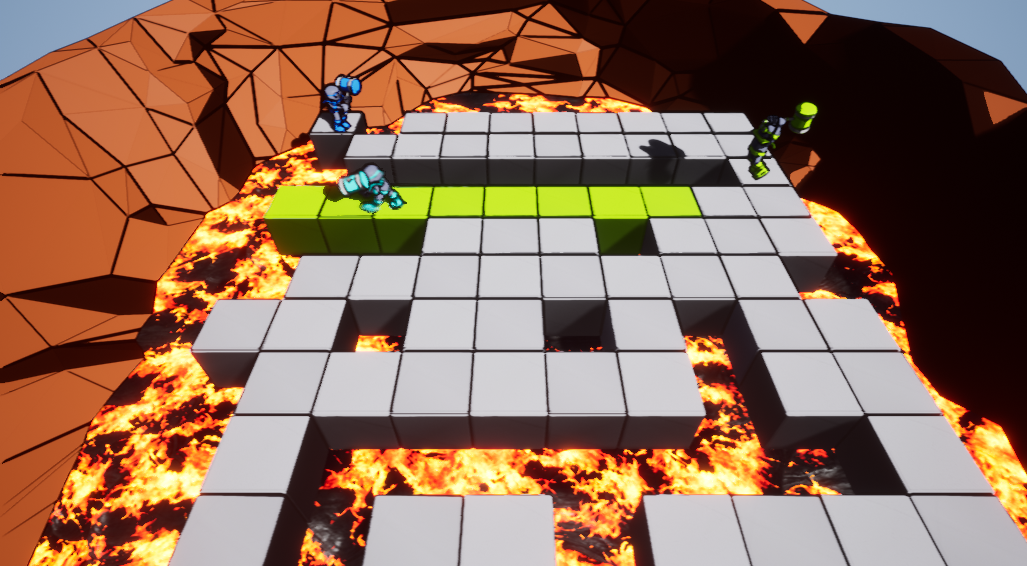
\includegraphics[width=\textwidth]{gameplay1.png}
\caption{3 Player Game-Play}
\end{figure}}]


%\maketitle


%
% paper title
% Titles are generally capitalized except for words such as a, an, and, as,
% at, but, by, for, in, nor, of, on, or, the, to and up, which are usually
% not capitalized unless they are the first or last word of the title.
% Linebreaks \\ can be used within to get better formatting as desired.
% Do not put math or special symbols in the title.
% \title{Game Design Functional Minimum\\Shattered}


% author names and affiliations
% use a multiple column layout for up to three different
% affiliations
%\author{\IEEEauthorblockN{Seth Miers}
%\IEEEauthorblockA{School of Electrical and\\Computer Engineering\\
%Univeristy of Colorado at Denver\\
%CSCI 5920 - Fall 2019\\
%Seth.Miers@UCDenver.EDU}
%}

% conference papers do not typically use \thanks and this command
% is locked out in conference mode. If really needed, such as for
% the acknowledgment of grants, issue a \IEEEoverridecommandlockouts
% after \documentclass

% for over three affiliations, or if they all won't fit within the width
% of the page (and note that there is less available width in this regard for
% compsoc conferences compared to traditional conferences), use this
% alternative format:
% 
%\author{\IEEEauthorblockN{Michael Shell\IEEEauthorrefmark{1},
%Homer Simpson\IEEEauthorrefmark{2},
%James Kirk\IEEEauthorrefmark{3}, 
%Montgomery Scott\IEEEauthorrefmark{3} and
%Eldon Tyrell\IEEEauthorrefmark{4}}
%\IEEEauthorblockA{\IEEEauthorrefmark{1}School of Electrical and Computer Engineering\\
%Georgia Institute of Technology,
%Atlanta, Georgia 30332--0250\\ Email: see http://www.michaelshell.org/contact.html}
%\IEEEauthorblockA{\IEEEauthorrefmark{2}Twentieth Century Fox, Springfield, USA\\
%Email: homer@thesimpsons.com}
%\IEEEauthorblockA{\IEEEauthorrefmark{3}Starfleet Academy, San Francisco, California 96678-2391\\
%Telephone: (800) 555--1212, Fax: (888) 555--1212}
%\IEEEauthorblockA{\IEEEauthorrefmark{4}Tyrell Inc., 123 Replicant Street, Los Angeles, California 90210--4321}}



% use for special paper notices
%\IEEEspecialpapernotice{(Invited Paper)}




% make the title area
%\maketitle

% As a general rule, do not put math, special symbols or citations
% in the abstract
%\begin{abstract}
%The abstract goes here.
%\end{abstract}

% no keywords




% For peer review papers, you can put extra information on the cover
% page as needed:
% \ifCLASSOPTIONpeerreview
% \begin{center} \bfseries EDICS Category: 3-BBND \end{center}
% \fi
%
% For peerreview papers, this IEEEtran command inserts a page break and
% creates the second title. It will be ignored for other modes.
% \IEEEpeerreviewmaketitle


\begin{abstract}
Shattered is a couch co-op fighting game. The goal is to break the blocks underneath your opponents to get them to fall off the map. The last person left standing on the map wins the round. The players can jump to get over gaps and they can slam their hammer into the blocks to break them.
\end{abstract}

\section{Project Webpage}

\subsection{Main Code}
https://github.com/superzanti/Shattered

\subsection{Compiled Release}
https://github.com/superzanti/Shattered/\\
releases/download/v0.5/\\
Shattered\_Winx64\_Alpha0.5.zip

\section{Core Strengths}

The game's core idea was to be a fun couch arena game with realistic physics. I believe it succeeded in both of these areas and anyone can pick up a controller and quickly understand the basic concept of the game.

\begin{figure*}[b]
  \centering
  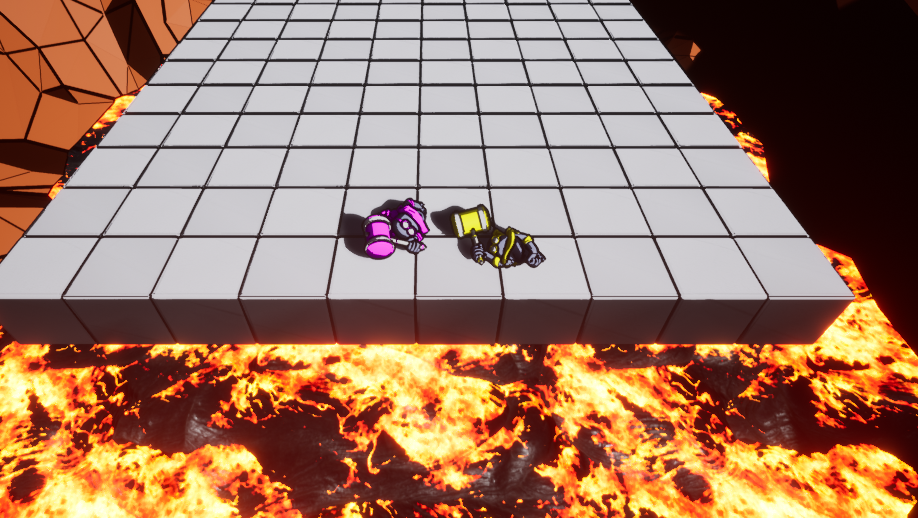
\includegraphics[width=0.8\textwidth]{simulated_ragdoll.png}%
  \caption{Fully Functional Ragdoll Physics}
\end{figure*}

\begin{figure*}[b]
  \centering
  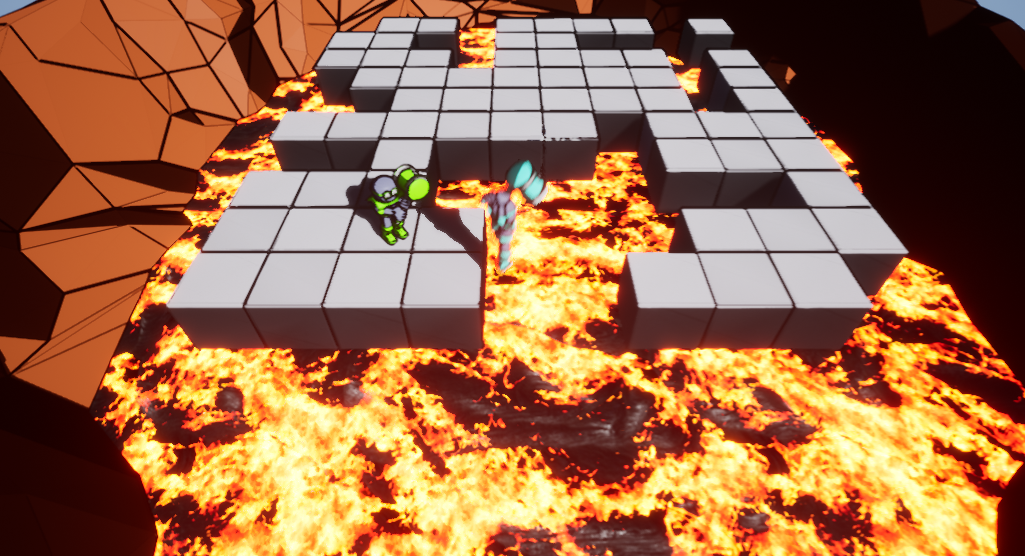
\includegraphics[width=0.8\textwidth]{jumping.png}%
  \caption{Tuned Jumping Physics}
\end{figure*}

% Fully Playable Game

\begin{figure*}[t]
  \centering
  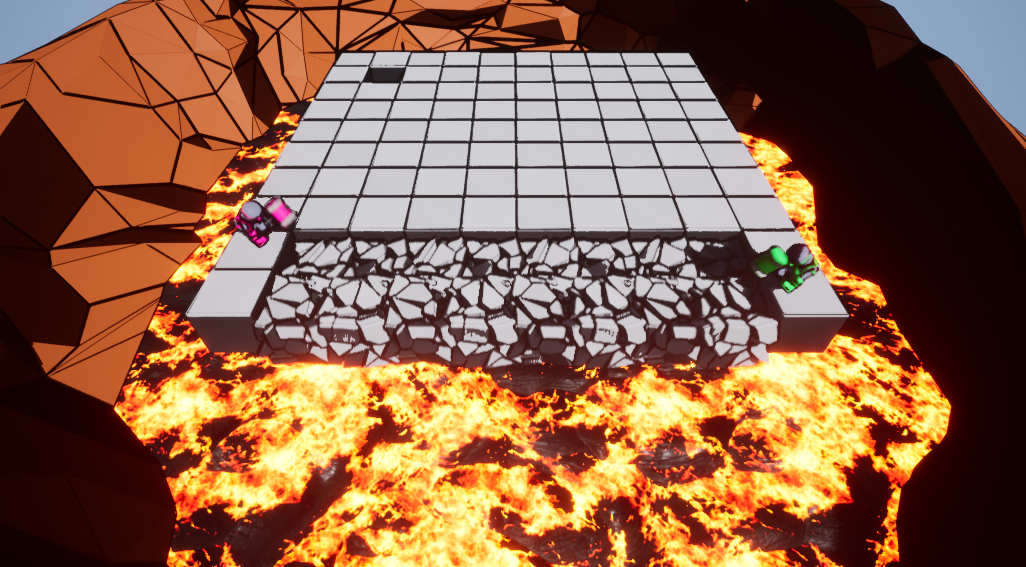
\includegraphics[width=0.8\textwidth]{blocksbreaking.png}%
  \caption{Physically Accurate Destructible Mesh for Blocks Breaking}
\end{figure*}
\begin{figure*}[b]
  \centering
  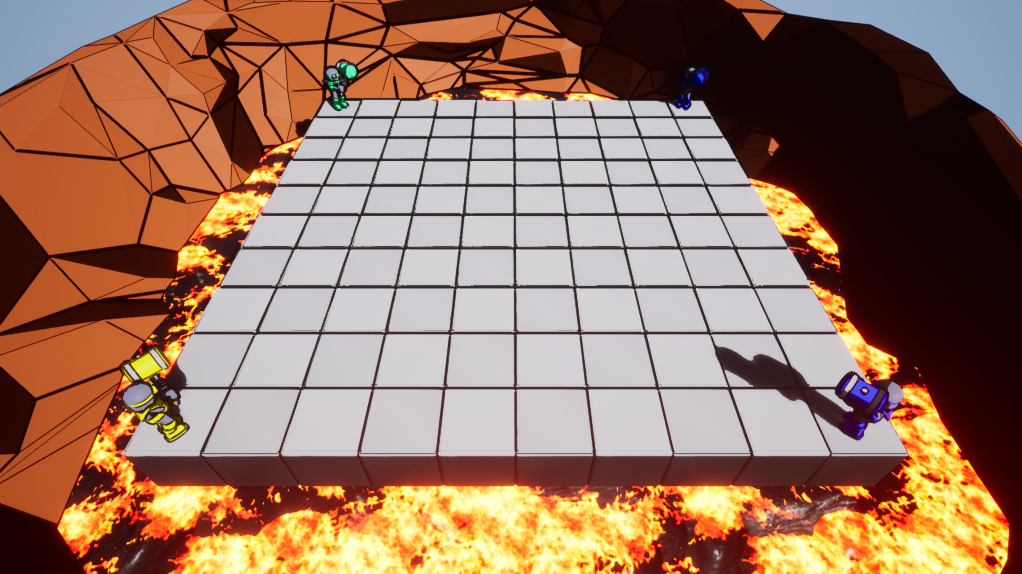
\includegraphics[width=0.8\textwidth]{spawns.png}%
  \caption{4 Total Spawn Points for Multiplayer Play}
\end{figure*}

\newpage
\subsection{Physics}

Physics was the main research component for this project. It ended up being implemented in a very nice way. The character has predictable movement speeds and realistic acceleration. All of the player controls are very tight, with controllable jump heights and animations that match what the character is doing.

Physics goes far beyond just a 'physics engine'. While that still has to be fought with to achieve desirable results, much of physics is simply in how the player views the character and not in what the character actually does.

This process started with the 3D model that would be used as the character. Realistic physics would not have been able to be achieved as well if it wasn't an object the player was familiar with. A humanoid was chosen for these reasons. The humanoid was then rigged such that realistic body physics could be achieved. This meant not skimping out on some bones that help the realism, while removing bones that are not necessary to achieve better optimization.

The animation then had to be done in a way that looked physically reasonable. This took reading, studying, and watching many slow-motion videos of walk and run cycles to make sure the character looked physically 'normal'. This whole process took much longer than expected.

The character was then textured and moved into unreal engine, where one of the next most important features was implemented: the player's physics asset. The balance between physically accurate and number of collision areas had to be compared and balanced. Constraints on every joint had to be set up so that the body would fall in a realistic manner as well. The result was a beautiful physics asset that would rag-doll properly and really enhanced the feel of realistic physics.

Beside the physics engine configuration, the animation, model, and rigging, the external environment also had to be configured properly. Correct physics simulations of blocks breaking can also be seen in this game. Even players interacting with each other had to be done in a realistic manner. Instead of a hard stop, like one would expect with most primitive unreal engine collision box, a custom collision box had to be made to account for 'soft' or 'bouncy' collisions.

\subsection{Fully Playable Game}

For the time allocated for this game, it is amazing that there is a fully playable release that can be enjoyed by a group of friends (or even strangers).

The game loops infinitely and it's always hard to say no to another round since they're so quick and easy to play. I found myself simply enjoying the character and running around every time I tested a new feature.

The game is elegant enough with the physics, that there are multiple levels of mastery. Due to the variable jump height, a character can jump a different length of blocks, they can do fake-out jumps, and they can even use the jump time as a strategy for messing with an opponent.

Variable run speeds also provide another level of control. Not only can you gain enough momentum to clear a gap, but you can walk slowly to get right up to the edge of a block for a quick escape.

While it's hard to pull off it is also very much possible to jump off another player's head. Every little aspect of this game comes down to a single point where it's simply just fun to play and fun to get distracted by.

The game even supports full  local multiplayer with up to 4 players. All players use a different gamepad. The game was tested with the USB Xbox 360 controller. This functionality can be seen in Figure 5.

\begin{figure*}[b]
  \centering
  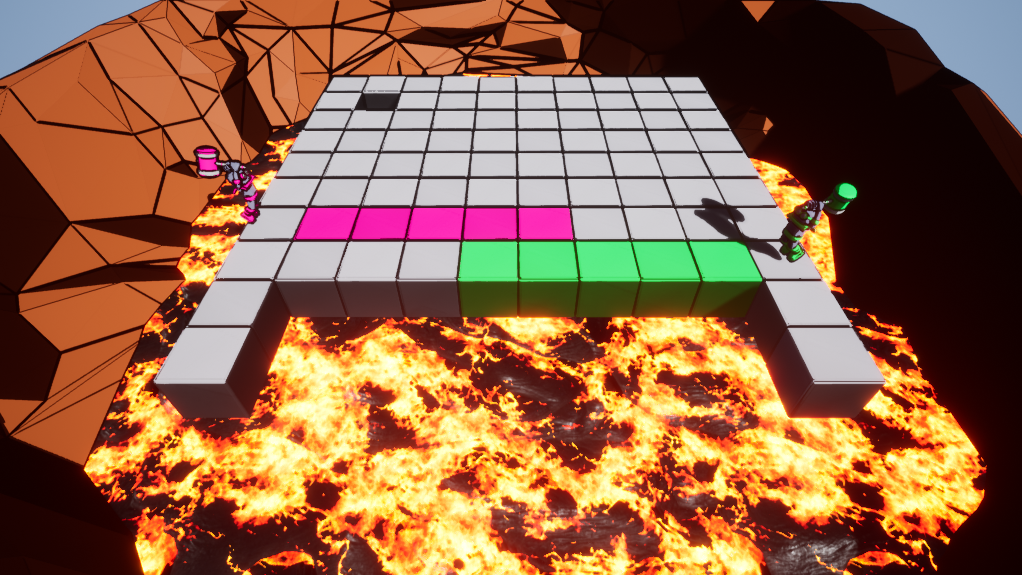
\includegraphics[width=0.8\textwidth]{blockscharging1.png}%
  \caption{Hammer Mode Charges Up So Player Can Break Multiple Blocks}
\end{figure*}

\subsection{All Asset Design}

Nothing in this game was borrowed, used, or stolen from someone else or even any other organization. Every asset, texture, animation, physics body, mesh, and more were all created by me.

While it doesn't show as a core strength at face value, once one realizes how much work goes into even just one asset of a game, this could be the biggest strength.

\section{Changes to Original Concept}

The overall concept of the game was kept the same throughout the duration of work. However, Many features were thought up during the development process, and many were sacrificed as a result of the time constraints.

\begin{figure*}[t]
  \centering
  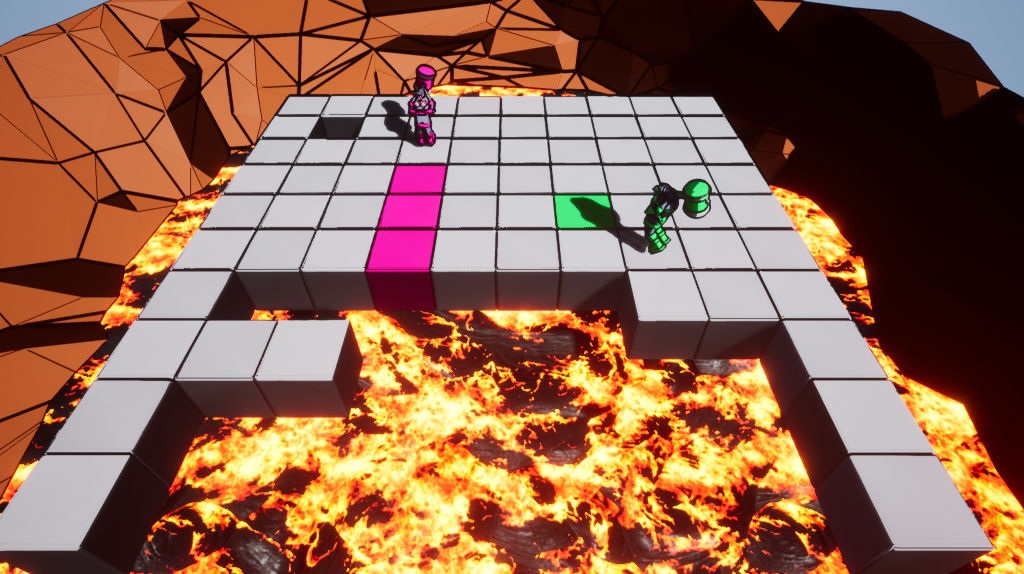
\includegraphics[width=0.8\textwidth]{blockscharging2.png}%
  \caption{Hammer Can Only Break 1 in the Diagonal, and Up To 8 In Horizontal or Vertical}
\end{figure*}

\subsection{Minimal Player Customization}

While modeling and playing with textures, I realized how easy it would be to make a dynamic material in Unreal Engine so that players could change the color of their character. This ended up being implemented very well.

Harder customization such as swap-able heads and hammers had their core functionality implemented. The character asset is designed to have 2 sockets that other meshes can connect to. One is the 'head' socket, and the other is the 'hammer' socket. Changing the color of these meshes was also achieved.

\subsection{Simple Menu Screen}

Without some kind of menu screen color customization would not be achievable, also there would always be 4 players on the screen. If you have only 3 controllers, there would still be another player spawned which could mess up how the game plays. It was chosen to add in a menu to make the game more playable.

\subsection{Audio}

No game is complete without audio. Without audio a game can be very bland and the player won't feel as connected to it. The choice to add audio was just so that the game would have a feeling of completeness.

\subsection{Block Breaking Options}

Originally the character could break as many blocks in any 360 degrees of direction. This ended up feeling weird and unpredictable since humans are unable to quickly determine which blocks will break in a certain direction. All 360 degrees of rotation also would decreased the strategy involved and it would end up playing as a 'quick draw' type of game. So the options on block breaking is limited to 1 in the diagonal or any number in the horizontal or vertical directions. This can be seen in Figure 6 and Figure 7.

\section{Play-ability Changes}

As the game grew, it became apparent that original ideas for how things would work would need to be changed in order to optimize the flow of the game. Many of these just had to do with how the player controlled their character and the pacing of the game itself.

\subsection{Physics Changes}

With the base physics, even having the character look moderately real, The character still felt too springy and hard to control. As it was it was possible for a character to jump over 5 blocks at once, which would make the game last forever and reduce the amount of strategy required. Physics were tuned to still be realistic but reduce the jump height to just one character in height, and friction was added to the air so that characters could only jump over 1 block easily, and 2 blocks if they were really experienced.

\begin{lstlisting}[caption={Biggest Physics Engine Tuning Parameters}]
GetCharacterMovement()->bOrientRotationToMovement = true;
GetCharacterMovement()->RotationRate = FRotator(0.f, 800.f, 0.f);
GetCharacterMovement()->bConstrainToPlane = true;
GetCharacterMovement()->bSnapToPlaneAtStart = true;
GetCharacterMovement()->MaxWalkSpeed = 1100.0f;
GetCharacterMovement()->MaxAcceleration = 10000.0f;
GetCharacterMovement()->JumpZVelocity = 800.0f;

GetCharacterMovement()->BrakingDecelerationFalling = 800.f;
GetCharacterMovement()->BrakingFriction = 0.5f;
GetCharacterMovement()->AirControl = 50.f;
GetCharacterMovement()->GravityScale = 2.2;
\end{lstlisting}

\subsection{Animation Speed}

While I wanted to show off the time I spent on the animation, it ended up being a big detriment to game-play. Jump animations were too slow and took too long from when the player clicked 'a' till the player jumped. The same problem was true when landing and swinging the hammer. Animations were sped up to feel fluid to the player and help the player feel as if they were in full control.

\section{Play-Testing}

The game was play tested several times throughout development, which is how many issues were found. However, the final test proved to be very beneficial. What I saw as a developer as needed to be fixed first, was a completely different priority from what the players thought should be changed first.

\subsection{Testers had Fun}

One group of play testers got carried away and kept starting new games. It was fun and exciting for them.

\textit{"It was fun. The rounds were quick and engaging. It was easy to keep jumping into the next round. I found there was more strategy to it than I had expected. Looked good. Felt good. Intuitive controls." -Elliot}

\textit{"The game was a lot of fun, and hard to put down. It’s great for small groups of friends, and results in a lot of laughs. The volcanic texture and the controller vibration were really cool. I liked being able to change the color of my avatar to any shade of the available colors." -Rachel}

All may play testers thought it was fun. So I consider that a huge success.

\begin{figure*}[t]
  \centering
  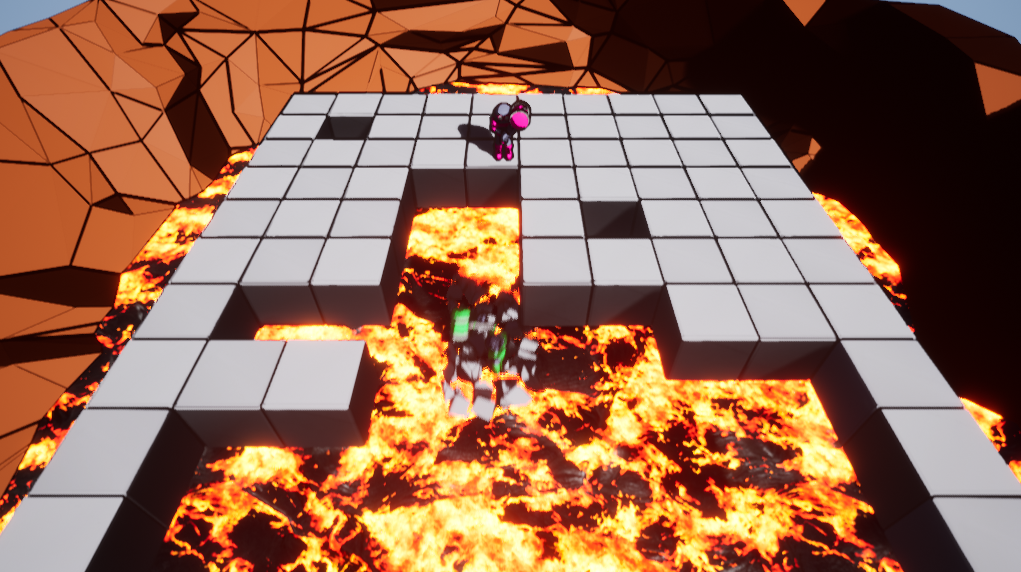
\includegraphics[width=0.8\textwidth]{dying.png}%
  \caption{Player Falling Off the Map and Ragdolling}
\end{figure*}
\begin{figure*}[b]
  \centering
  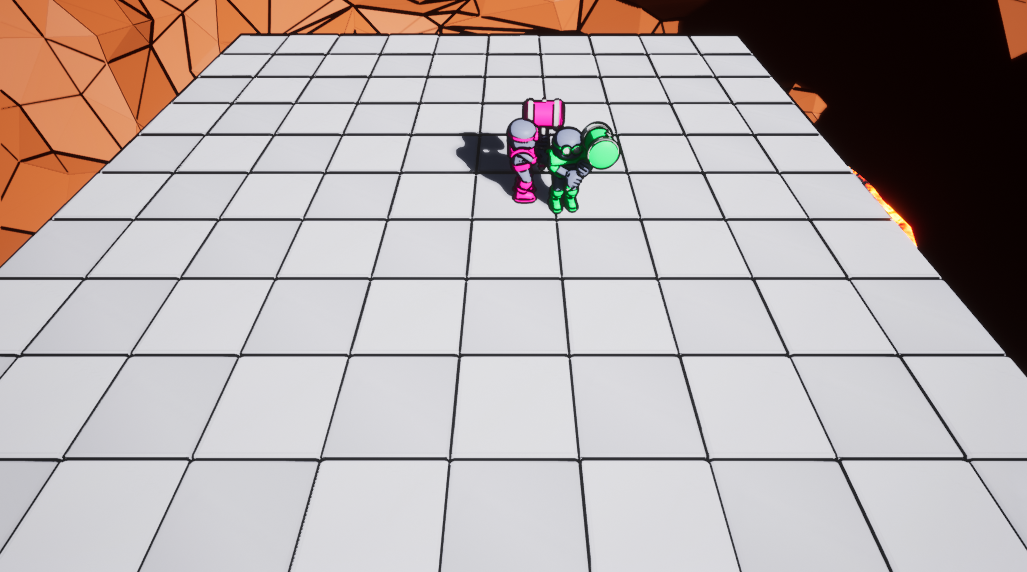
\includegraphics[width=0.8\textwidth]{zoom1.png}\\~\\
  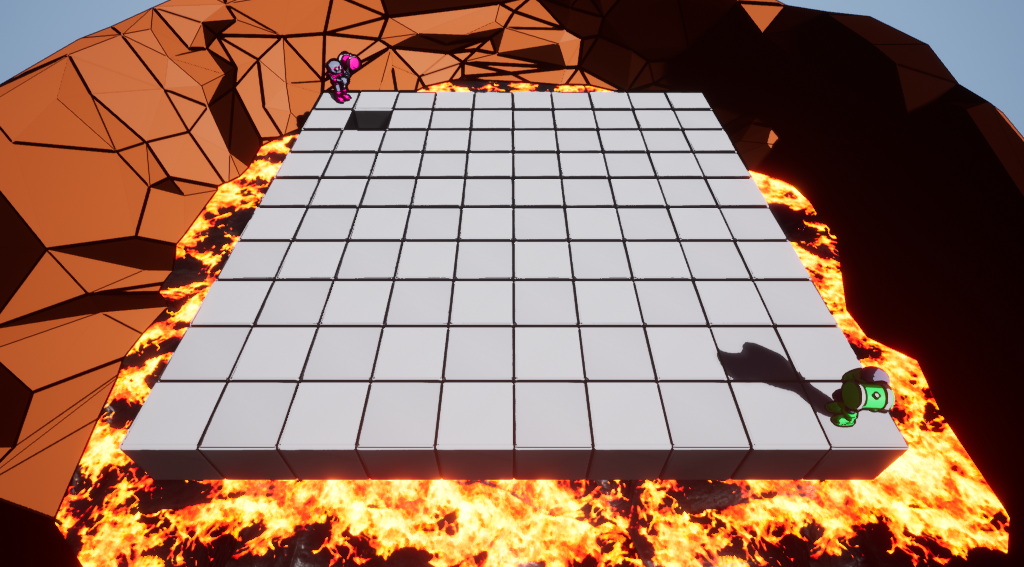
\includegraphics[width=0.8\textwidth]{zoom2.png}%
  \caption{Camera Position and Zoom Levels Based on Player Position}
\end{figure*}
\begin{figure*}[b]
  \centering
  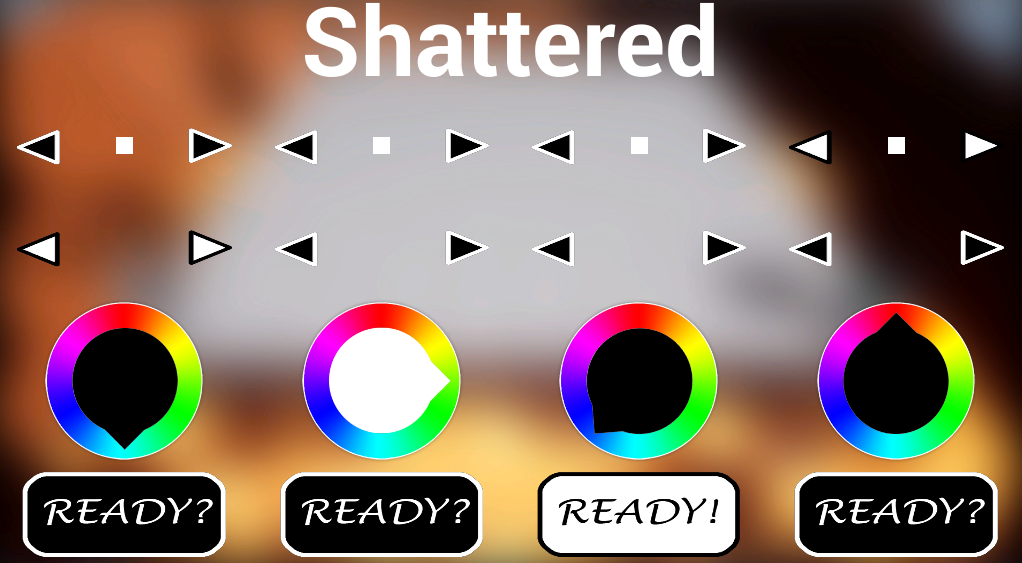
\includegraphics[width=0.8\textwidth]{mainmenu.png}%
  \caption{Fully implemented Main Menu and Player Customization}
\end{figure*}
\begin{figure*}[b]
  \centering
  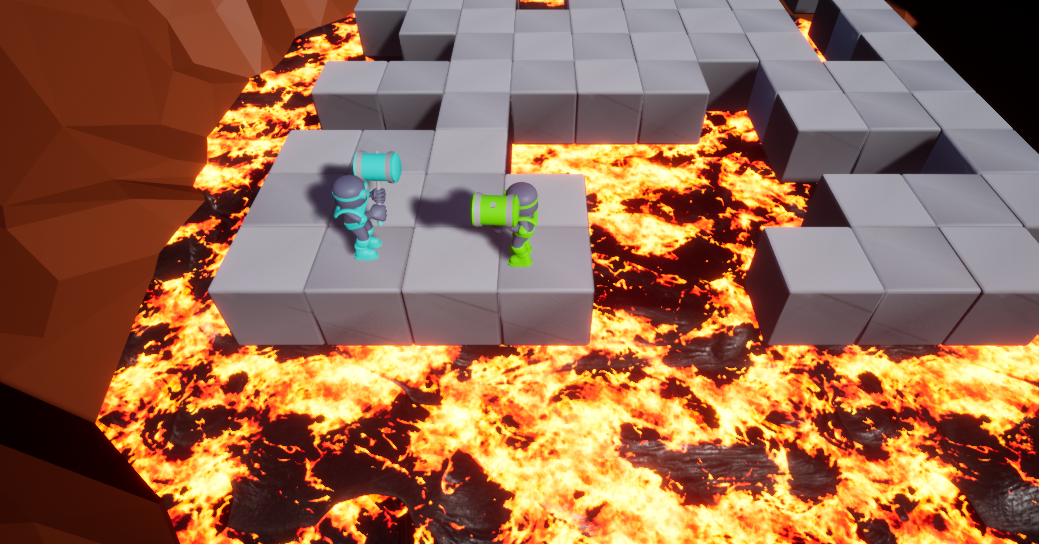
\includegraphics[width=0.8\textwidth]{cell_shading_disabled.png}%
  \caption{Cell Shading and Outline Disabled}
\end{figure*}

\subsection{Bugs Galore}

The players also had fun finding small bugs. As one player stated 'there is nothing game braking'. Many of the bugs are simply funny or just something that makes one go 'oops'.

\textit{"The main menu looked a little incomplete, but it's functional. There are probably a few bugs that still need to be worked out, but nothing game breaking. I think there needs to be some thought put into preventing/resolving potential stalemate scenarios, like random blocks breaking after a certain amount of time" -Elliot}

\textit{"The time it takes to charge the hammer is a bit long, but that doesn’t impede game-play or enjoyment too much." -Rachel}

\section{Testing Changes}
Since many of the bugs could not be fixed within the time-frame, my focus was directed to the game-play itself.

\subsection{Player Movement}

The acceleration had to be tuned. Some players found that quickly turning around resulted in a total loss of momentum, and while this is physically accurate, it leaded to them feeling like they were being cheated by the game instead of being in control of their character. The max acceleration of a character was tuned so that a character could quickly turn around and have enough momentum to jump over one block.
The speed of the hammer charge rate was also tuned. I found through testing that players ended up using the single block hammer the most because it gave other players less time to react.

\subsection{Collisions}

When trying to tune the physics for the rag-doll and the effect for landing on lava, I ended up breaking the collisions for the destructible meshes used for the blocks. Players found that they could still jump off of blocks as they were falling. This made it hard to feel like you were eliminating another player and made it instead feel like you were just trying to survive the longest without mistakes. Fixing these collisions fixed that problem.

\section{Time Constraints}

The biggest problem in the entire project was time constraints. As the project progressed I learned that every single component takes way longer than I thought it would. It gave me a huge appreciation for many of the games that come out today. Hours were spent on just tuning one physics component, days were spent on the overall physics, hours again were spent on modeling and animation. The list goes on and on. I slowly began to realize that my goals were too lofty for the time allowed. While this could be a fully polished game with another work-weeks of work, I simply didn't have another set of 40 hours to spend on the game.

\subsection{Achievements and Score Tracking}

Achievements and score tracking would've taken too much time to implement and I prioritized having a functional game. Post screen achievements and stats would have made the game really enjoyable and definitely more competitive, but in the end, the game-play was much more important.

\subsection{Audio}

Some of the functionality for audio was there, but I did not have the time to make my own sounds, and it was important to me that every single part of this game was made and designed by myself. For footsteps I did not have time to set up a mic and record sounds, however, the controller does slightly vibrate every time the character steps as a drop in replacement (and maybe addition because everyone really liked it).
Game music was not implemented as composing songs takes hours alone.

\subsection{Code Organization}

Rushing to get a complete project done within the time frame lead to some bad coding practices. If I had more time I would go back and re-organize where much of the code is, add in comments, and add variables where variables are needed. I found myself having to change code in 3 places at the end when I wanted to change something.

\section{Lessons Learned}

In the future I would also get a broader range of play testers. Having just friends and family limits the feedback. I fear that many of them are too scared to say much that is bad about the game.

\subsection{Physics is Difficult}

Getting physics to look correct while also making sure the game-play still feels good is  extremely difficult. There was also much difficulty in figuring out how to fight the built in Unreal Physics Engine. Many of the commands I had to use were hard to find in documentation such as AirControl and BrakingFriction.

\subsection{Time Estimation}

The biggest lesson I learned was how long everything takes. Stuff I've already done, I'm sure I could do faster the next time around, but in general, It takes much longer to do one thing, and you will always run into problems. Sometimes it's a missing vertex, a face that's too small, a joint that won't move right, a collision that won't trigger, or any other hundreds of things, but there are always small issues that will take much longer to fix than if everything had just gone perfectly the first time.

\subsection{Code Organization}

Since I plan to work on this game in the future and add in some final polish, it would have been very beneficial to maintain the code in a very meticulous manner. Even though it would have come with the sacrifice of not having a full game to submit, it would have made my life easier in the future.
It's always better to put in the work to have good project organization ahead of time.

%\begin{figure*}
%  \centering
%  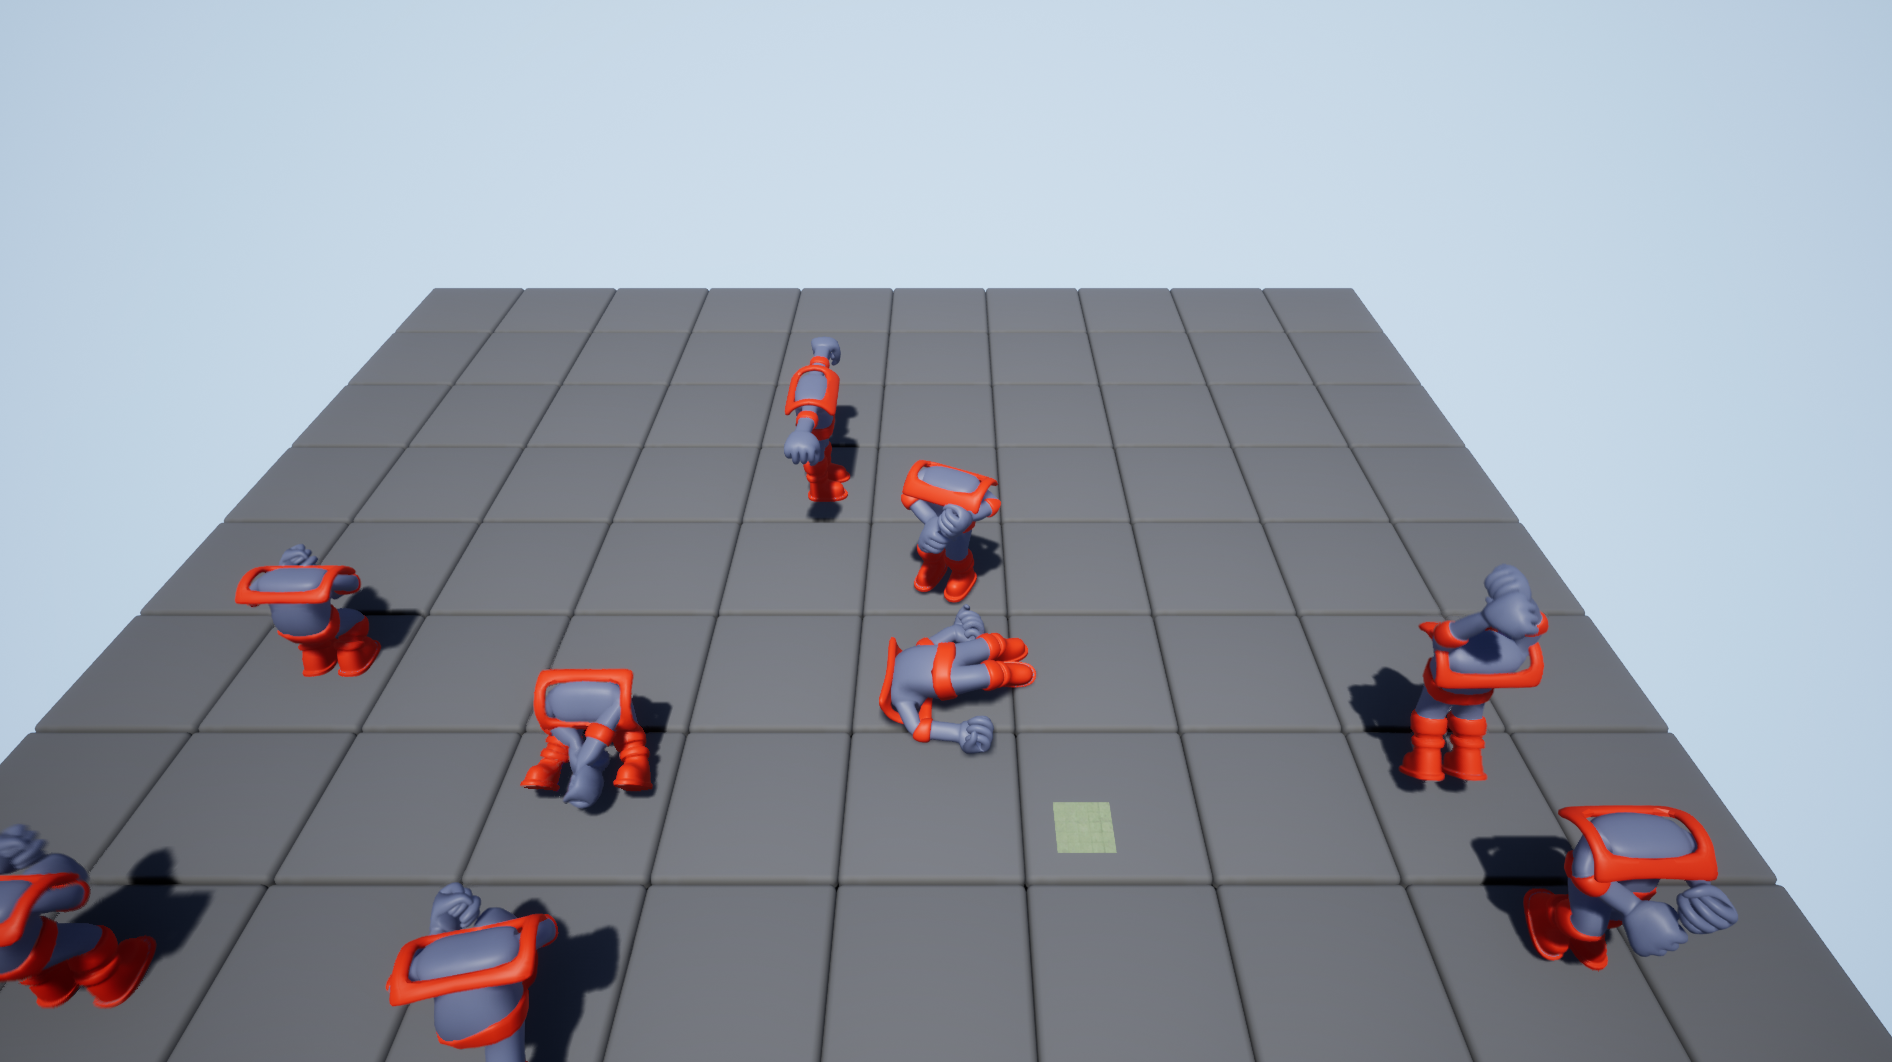
\includegraphics[width=\textwidth]{maingame.png}
%  \caption{First demo release}
%\end{figure*}
%\newpage
%
%\begin{figure}[h]
%\centering
%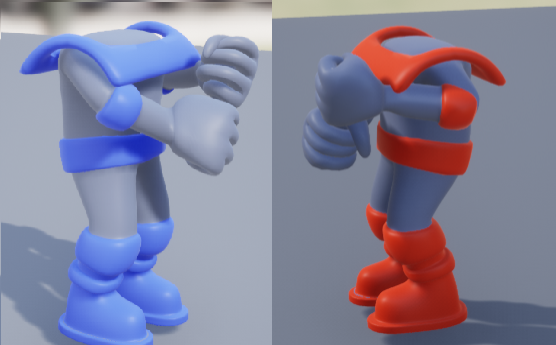
\includegraphics[width=2.5in]{2colors.png}
%\caption{Quickly hot-swapable colors}
%\label{fig_sim}
%\end{figure}
%
%\begin{figure}[h]
%\centering
%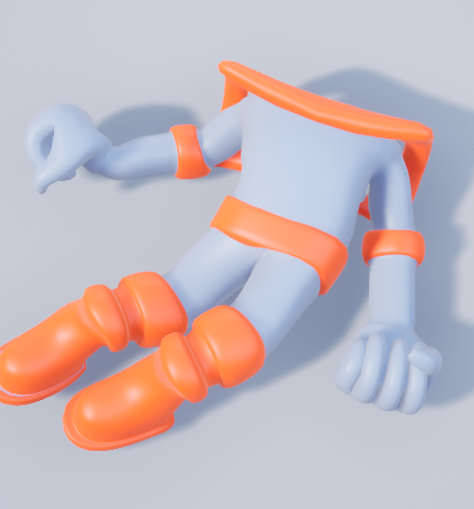
\includegraphics[width=2.5in]{limpbody.png}
%\caption{The body falls limp in a realistic way}
%\label{fig_sim}
%\end{figure}

% An example of a floating figure using the graphicx package.
% Note that \label must occur AFTER (or within) \caption.
% For figures, \caption should occur after the \includegraphics.
% Note that IEEEtran v1.7 and later has special internal code that
% is designed to preserve the operation of \label within \caption
% even when the captionsoff option is in effect. However, because
% of issues like this, it may be the safest practice to put all your
% \label just after \caption rather than within \caption{}.
%
% Reminder: the "draftcls" or "draftclsnofoot", not "draft", class
% option should be used if it is desired that the figures are to be
% displayed while in draft mode.
%
%\begin{figure}[!t]
%\centering
%\includegraphics[width=2.5in]{myfigure}
% where an .eps filename suffix will be assumed under latex, 
% and a .pdf suffix will be assumed for pdflatex; or what has been declared
% via \DeclareGraphicsExtensions.
%\caption{Simulation results for the network.}
%\label{fig_sim}
%\end{figure}

% Note that the IEEE typically puts floats only at the top, even when this
% results in a large percentage of a column being occupied by floats.


% An example of a double column floating figure using two subfigures.
% (The subfig.sty package must be loaded for this to work.)
% The subfigure \label commands are set within each subfloat command,
% and the \label for the overall figure must come after \caption.
% \hfil is used as a separator to get equal spacing.
% Watch out that the combined width of all the subfigures on a 
% line do not exceed the text width or a line break will occur.
%
%\begin{figure*}[!t]
%\centering
%\subfloat[Case I]{\includegraphics[width=2.5in]{box}%
%\label{fig_first_case}}
%\hfil
%\subfloat[Case II]{\includegraphics[width=2.5in]{box}%
%\label{fig_second_case}}
%\caption{Simulation results for the network.}
%\label{fig_sim}
%\end{figure*}
%
% Note that often IEEE papers with subfigures do not employ subfigure
% captions (using the optional argument to \subfloat[]), but instead will
% reference/describe all of them (a), (b), etc., within the main caption.
% Be aware that for subfig.sty to generate the (a), (b), etc., subfigure
% labels, the optional argument to \subfloat must be present. If a
% subcaption is not desired, just leave its contents blank,
% e.g., \subfloat[].


% An example of a floating table. Note that, for IEEE style tables, the
% \caption command should come BEFORE the table and, given that table
% captions serve much like titles, are usually capitalized except for words
% such as a, an, and, as, at, but, by, for, in, nor, of, on, or, the, to
% and up, which are usually not capitalized unless they are the first or
% last word of the caption. Table text will default to \footnotesize as
% the IEEE normally uses this smaller font for tables.
% The \label must come after \caption as always.
%
%\begin{table}[!t]
%% increase table row spacing, adjust to taste
%\renewcommand{\arraystretch}{1.3}
% if using array.sty, it might be a good idea to tweak the value of
% \extrarowheight as needed to properly center the text within the cells
%\caption{An Example of a Table}
%\label{table_example}
%\centering
%% Some packages, such as MDW tools, offer better commands for making tables
%% than the plain LaTeX2e tabular which is used here.
%\begin{tabular}{|c||c|}
%\hline
%One & Two\\
%\hline
%Three & Four\\
%\hline
%\end{tabular}
%\end{table}


% Note that the IEEE does not put floats in the very first column
% - or typically anywhere on the first page for that matter. Also,
% in-text middle ("here") positioning is typically not used, but it
% is allowed and encouraged for Computer Society conferences (but
% not Computer Society journals). Most IEEE journals/conferences use
% top floats exclusively. 
% Note that, LaTeX2e, unlike IEEE journals/conferences, places
% footnotes above bottom floats. This can be corrected via the
% \fnbelowfloat command of the stfloats package.



%\section{Conclusion}
%The conclusion goes here.




% conference papers do not normally have an appendix



%% use section* for acknowledgment
%\ifCLASSOPTIONcompsoc
%  % The Computer Society usually uses the plural form
%  \section*{Acknowledgments}
%\else
%  % regular IEEE prefers the singular form
%  \section*{Acknowledgment}
%\fi
%
%
%The authors would like to thank...





% trigger a \newpage just before the given reference
% number - used to balance the columns on the last page
% adjust value as needed - may need to be readjusted if
% the document is modified later
%\IEEEtriggeratref{8}
% The "triggered" command can be changed if desired:
%\IEEEtriggercmd{\enlargethispage{-5in}}

% references section

% can use a bibliography generated by BibTeX as a .bbl file
% BibTeX documentation can be easily obtained at:
% http://mirror.ctan.org/biblio/bibtex/contrib/doc/
% The IEEEtran BibTeX style support page is at:
% http://www.michaelshell.org/tex/ieeetran/bibtex/
%\bibliographystyle{IEEEtran}
% argument is your BibTeX string definitions and bibliography database(s)
%\bibliography{IEEEabrv,../bib/paper}
%
% <OR> manually copy in the resultant .bbl file
% set second argument of \begin to the number of references
% (used to reserve space for the reference number labels box)
%\begin{thebibliography}{1}
%
%\bibitem{IEEEhowto:kopka}
%H.~Kopka and P.~W. Daly, \emph{A Guide to \LaTeX}, 3rd~ed.\hskip 1em plus
%  0.5em minus 0.4em\relax Harlow, England: Addison-Wesley, 1999.
%
%\end{thebibliography}
%
%\begin{appendices}
%\section{Some Appendix}
%The contents...
%\section{Some 2}
%\end{appendices}


%intentional blank end page
%\afterpage{\blankpage}
%\newpage
%\mbox{}
\newpage
\mbox{}
\newpage
\mbox{}
\addtocounter{page}{-1}
\thispagestyle{empty}

% that's all folks
\end{document}


